\title{Capstone project report: Estimate error from Zillow's home value prediction}
\author{
	Yun Zhang \\
}
\date{\today}
\documentclass[12pt]{article}
\usepackage{sectsty}
\usepackage{amsfonts,graphicx,amssymb,amsmath}
\usepackage{enumitem}
\sectionfont{\fontsize{14}{20}\selectfont}
\subsectionfont{\fontsize{12}{20}\selectfont}
\begin{document}
\maketitle

\section{Project definition}\label{sec:definition}
\subsection{Project overview}
Home value prediction is an efficient way to represent the general information for homes, which is important for both buyers and sellers to understand the housing market and monitor the values of their properties. The online real estate database company Zillow provides its own home value prediction (Zestimate) to help consumers predict home value at no cost. The 'Zestimate' estimates home values according to 7.5 million statistical and machine learning models that analyze hundreds of data points on each property. The Zillow company keeps improving their 'Zestimate', and its current median margin of error compared to the real sale price has dropped from 20\% to 5\% during the last 11 years. However, even though the prediction has a relatively high accuracy in percentage (95\%), due to the high total price of each property, the error in price prediction is still large enough to affect its reliability especially for buyers who need to apply for financial loan based on accurate home value.

The question is whether the 'Zestimate' can be further improved for higher accuracy and reliability. This is an interesting and important topic not only for the company but also any buyer or seller. In order to achieve this goal, it is necessary to evaluate the performance of the existing 'Zestimate' and find the weak point of the current algorithm. In this project, different machine learning techniques will be applied to build a predictive model that estimates the error between the 'Zestimate' and real sale price according to the information of each property. The predictive model can quantitatively analyze how the performance of 'Zestimate' varies under different scenarios for different properties, determines the key factors or features which induce errors due to the possible inadequate representation in the current 'Zestimate', and helps improving the design of a new algorithm for home value prediction.

\subsection{Problem statement}
In this project, different features of a home will be applied to estimate the log error ($\xi_{\log}$) between 'Zestimate' and real sale price. Here the log error is defined by

\begin{equation}
\xi_{\log}=\log(P_{zest})-\log(P_s)~\text{,}
\label{eq:define-log-error}
\end{equation}
where $P_{zest}$ is the price provided by 'Zestimate' while $P_s$ is the real sale price for a property. The problem is clearly a regression problem, which predicts the log error by the basic information for each house. The input may include multiple features like house location, home size, tax information and facilities. This problem may be solved by many regression techniques including linear regression, $k$ nearest neighbors and regression by decision tree and different boosting techniques.

\subsection{Performance metrics}
The mean absolute error (MAE) between the predicted and actual $\xi_{\log}$ (defined by Eqn. \ref{eq:define-log-error}) is applied as the evaluation metrics, which is defined as 

\begin{equation}
M=\frac{1}{N}\sum_{i=1}^{N}\left|\xi_{\log,pred}-\xi_{\log,real}\right|~\text{,}
\label{eq:define-evaluation-metric}
\end{equation}
where $N$ is the number of test data. The lower MAE will indicate a better prediction by the predictive model.

\section{Data analysis}\label{sec:analysis}
\subsection{Dataset overview}
The dataset includes two portions, a full list of real estate properties data and the completed transactions in three counties (Los Angeles, Orange and Ventura, California) during 2016. It is provided by Zillow for the Zillow prize competition held on the Kaggle platform (https://www.kaggle.com/c/zillow-prize-1). The first portion of the dataset provides the basic information for 2985217 houses. For each house, this portion provides information of 58 numeric and categorical features. All the features will be treated as the input for the predictive model to estimate $\xi_{\log}$. On the other hand, the second portion of the dataset provides the sale date and $\xi_{\log}$ of 90811 transactions for all houses sold within year 2016. The original dataset has already been split into training and test portions. The training data has all the transactions before October 15, 2016, plus some of the transactions after October 15, 2016. The rest of data forms the test dataset. Since the dataset is provided for an online competition, the test dataset is not accessible from the Kaggle platform to avoid cheating and abuse.

\subsection{Data exploration}
The first portion of the dataset provides the basic information for 2985217 houses at Los Angeles, Orange County and Ventura, California. Each house has 58 different features from the perspective of the property ID, location, home size (living area, lot size, garage size, etc.), tax information and facility types. For the data types, there are 2 features as string type and 56 numerical features with 17 categorical variables. Figure \ref{fig:missing-values} shows the percentage of missing values for each feature in this portion of dataset. All the features have missing values with the missing rate ranging from 0.38\% to 99.4\%, and there are 32 features with more than 50\% missing rate. This indicates filling the missing values may be necessary to maintain enough feature for the training purpose of the predictive model.

The second portion is the transaction dataset that provides the information of all the completed transactions before October and some tractions after October during 2016. For each transaction, there are only 3 features including the property ID, transaction date, the exact $\xi_{\log}$ between the 'Zestimate' and the real sale price. No missing values occur in this portion of dataset. According to the property ID, the portion of dataset can be merged with the house information to form the complete dataset for training dataset. According to the dataset, 127 houses have been sold for twice and 1 house has been sold for three times during 2016. More details between relationship among $\xi_{\log}$, transaction date, location and yearbuilt of each house will be discussed in the next section.

\begin{figure}[!ht]
	\centering
	\includegraphics[width=1\linewidth]{pic/missing-value}
	\caption{The percentage of missing values for different features of each house.}
	\label{fig:missing-values}
\end{figure}

\subsection{Exploratory visualization analysis}
\subsubsection{The number of sold house vs. sale month}
According to the transaction dataset, Figure \ref{fig:num-sold-vs-month} shows the histogram of the number of sold houses during different months of year 2016. Since the transaction dataset excludes the test data for October, November and December of year 2016, the number of sold houses decreases obviously in these three months. Generally more transactions occurred in the middle of the year (June), the maximum number of transactions can be nearly twice the number of houses sold in January.
\begin{figure}[!ht]
	\centering
	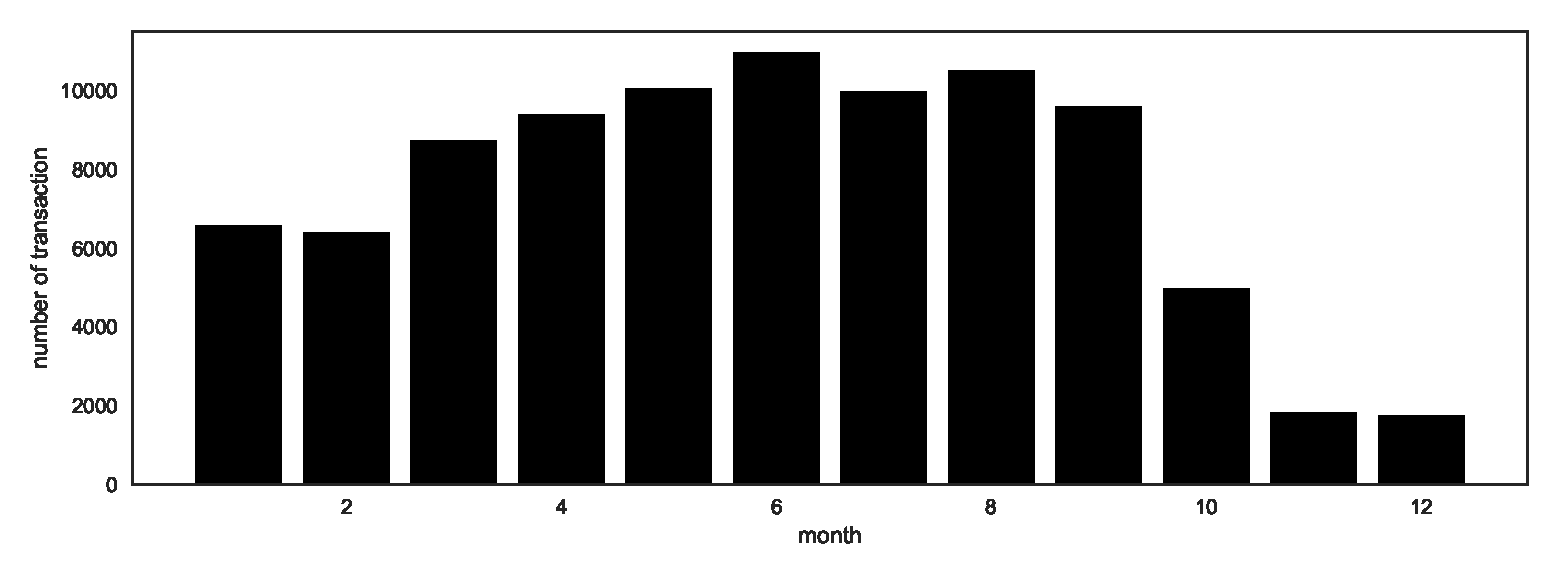
\includegraphics[width=1\linewidth]{pic/num-sold-vs-month}
	\caption{The histogram of sold houses in the transaction dataset during 2016.}
	\label{fig:num-sold-vs-month}
\end{figure}

\begin{figure}[!ht]
	\centering
	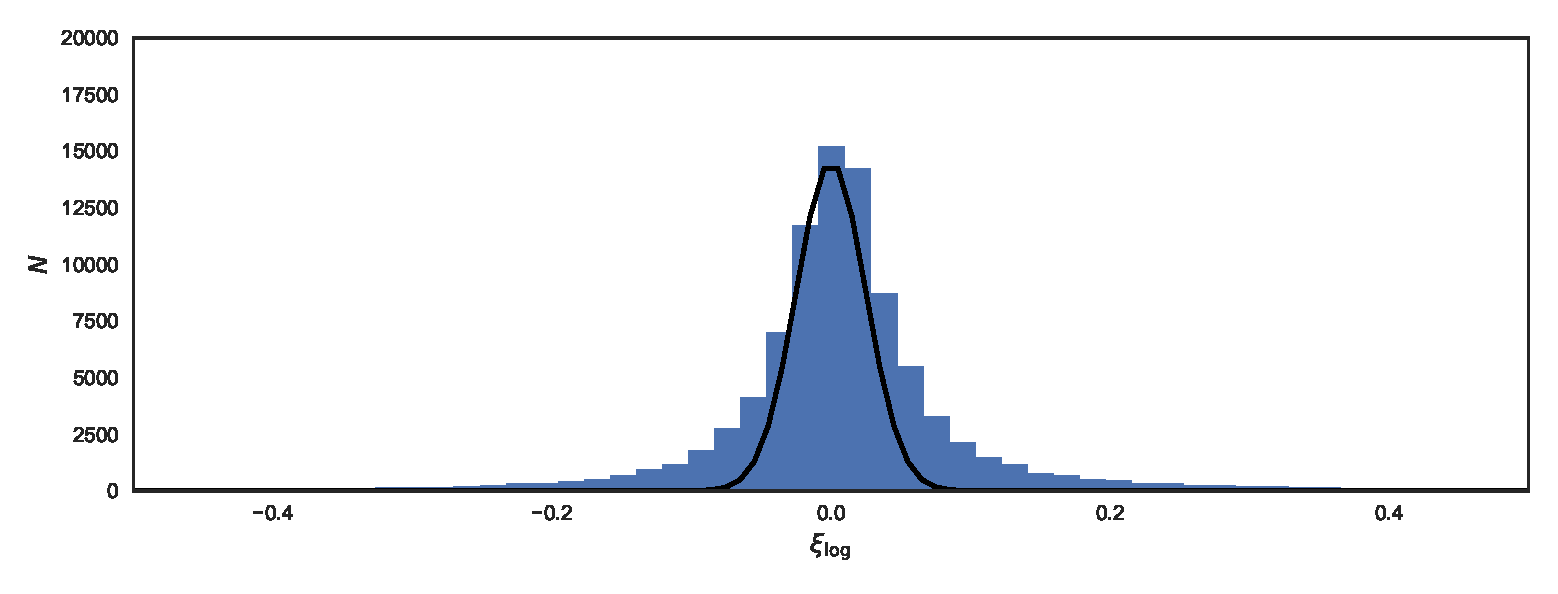
\includegraphics[width=0.9\linewidth]{pic/hist-error}
	\caption{The histogram of $\xi_{\log}$ in the transaction dataset. The solid line is the best fit of normal distribution.}
	\label{fig:hist-error}
\end{figure}

\subsubsection{The histogram of $\xi_{\log}$}
The histogram of $\xi_{\log}$ is shown by Figure \ref{fig:hist-error}. The comparison to the best fit of normal distribution indicates that the distribution of $\xi_{\log}$ does not follow normal distribution although the distribution has a similar shape.  

\begin{figure}[!ht]
	\centering
	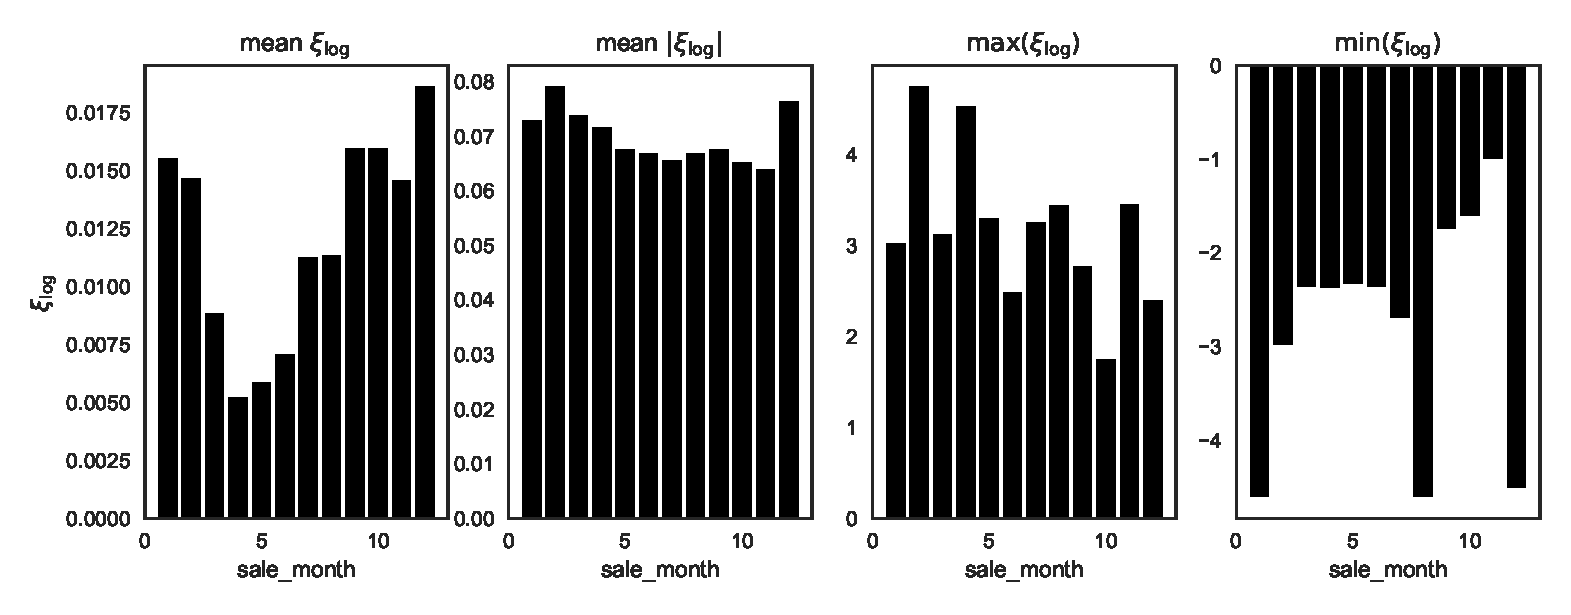
\includegraphics[width=1\linewidth]{pic/error-vs-month}
	\caption{The variations of monthly averaged $\xi_{\log}$, averaged $|\xi_{\log}|$, maximum and minimum $\xi_{\log}$.}
	\label{fig:error-vs-month}
\end{figure}


\begin{figure}[!ht]
	\centering
	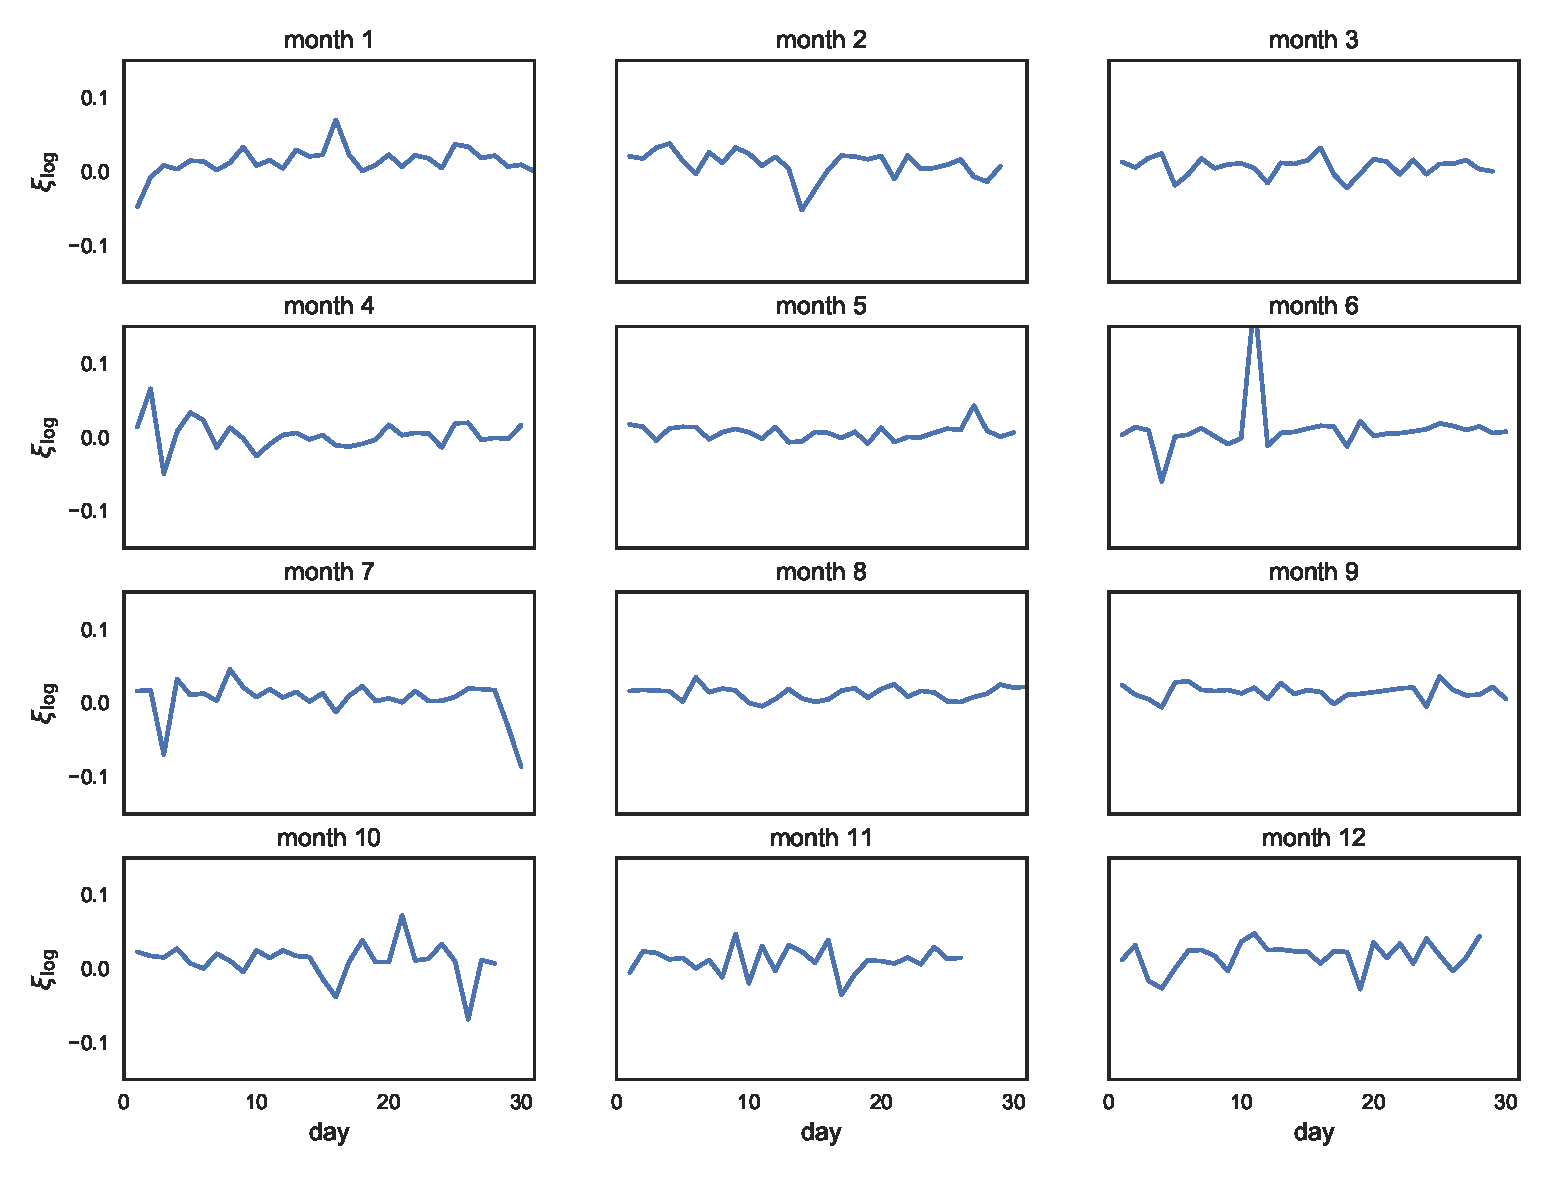
\includegraphics[width=0.9\linewidth]{pic/error-variation-different-month}
	\caption{The variations of $\xi_{\log}$ for transactions occured at different month during 2016.}
	\label{fig:error-variation-different-month}
\end{figure}

\begin{figure}[!ht]
	\centering
	\includegraphics[width=0.8\linewidth]{pic/error-long-lat}
	\caption{The spacial distribution of $\xi_{\log}$.}
	\label{fig:error-long-lat}
\end{figure}

\begin{figure}[!ht]
	\centering
	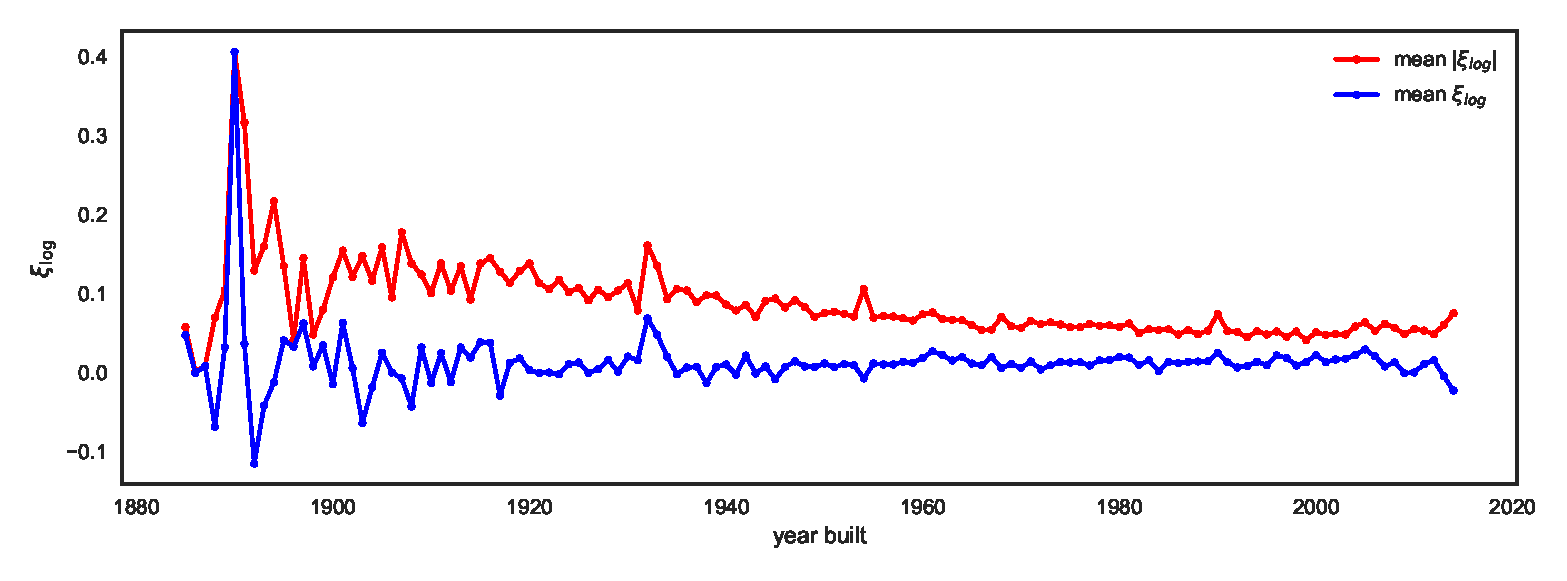
\includegraphics[width=0.85\linewidth]{pic/total-error-yearbuilt}
	\caption{The variations of $\xi_{\log}$ for houses that are built at different years.}
	\label{fig:total-error-yearbuilt}
\end{figure}

\begin{figure}[!ht]
	\centering
	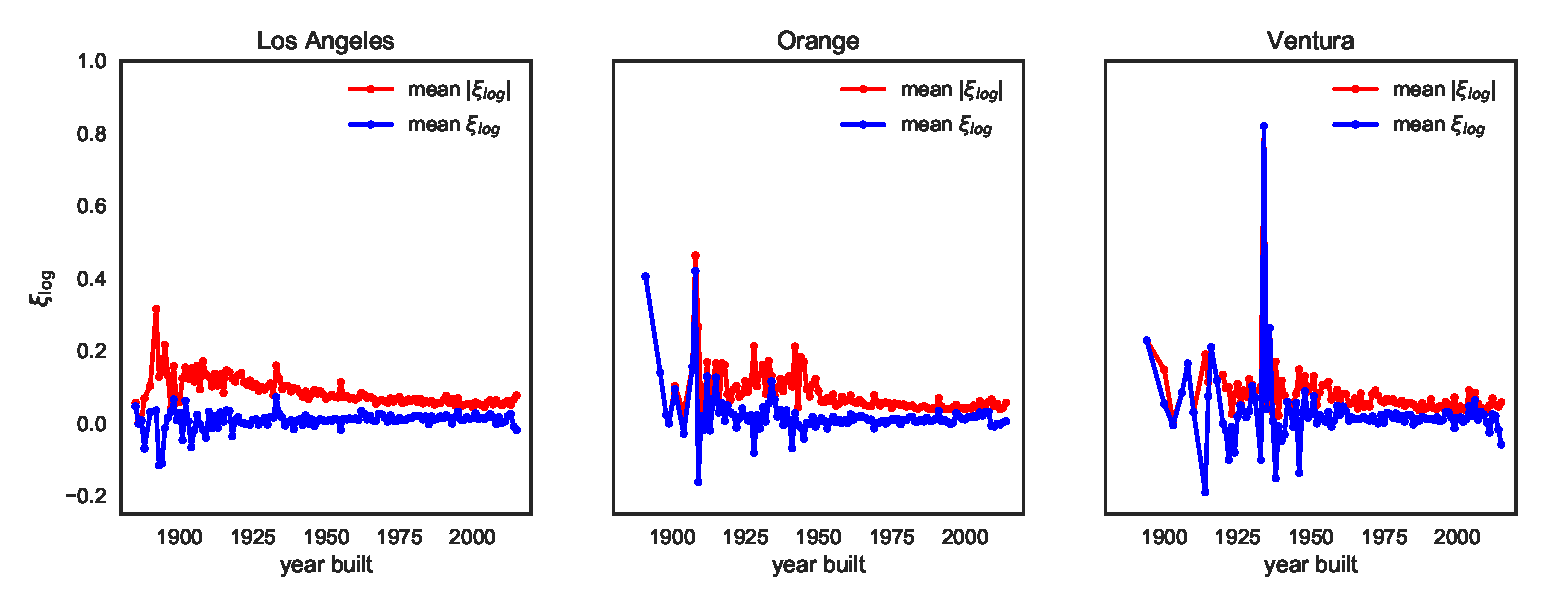
\includegraphics[width=1\linewidth]{pic/diff-location-error-yearbuild}
	\caption{The variations of $\xi_{\log}$ for houses that are built at different years for the three counties in California.}
	\label{fig:diff-location-error-yearbuild}
\end{figure}

\subsubsection{Transaction date vs. $\xi_{\log}$}
Figure \ref{fig:error-vs-month} shows the variations of monthly averaged $\xi_{\log}$, monthly averaged $|\xi_{\log}|$, maximum and minimum $\xi_{\log}$ during 2016. The range of $\xi_{\log}$ is from -4.6 to 4.7. Based on this figure, the $Zestimate$ performs better during April to August due to relative low mean $\xi_{\log}$. However, the mean absolute error shows a relative stable pattern and indicates that there is no different in the performance of $Zestimate$ at different month of year 2016. The variation of daily average $\xi_{\log}$ of different months in year 2016 has been shown by Figure \ref{fig:error-variation-different-month}. The shape of the variation of log error within each month is not obvious to indicate difference in months. But larger error occurs in June, July and October.

\subsubsection{The relationship among $\xi_{\log}$, house location and yearbuilt}
As shown by Figure \ref{fig:error-long-lat}, the spacial distribution of $\xi_{\log}$ does not show an obvious pattern and indicates that longitude and latitude are not the only factors that affect the performance of $Zestimate$. On the other hand, the yearbuilt of each sold house is another important factor to predict $\xi_{\log}$. According to Figure \ref{fig:total-error-yearbuilt}, large $\xi_{\log}$ occurs for houses built before year 1920, and the performance of 'Zestimate' is better and more stable for houses built after year 1940. Figure \ref{fig:diff-location-error-yearbuild} demonstrates how the relationship between $\xi_{\log}$ and house yearbuilt varies at three different counties of California. The pattern for Los Angeles is similar as the general shape in Figure \ref{fig:total-error-yearbuilt}, while large error occurs for houses built from year 1925 to 1950 at Orange county and Ventura. 
 
\subsection{Regression models}
Since the $\xi_{\log}$ prediction is a regression problem, the solution basically includes two steps which are data preprocessing and the optimization of regression model. In this project, six different regression models will be applied to predict $\xi_{\log}$,  The five regression models include linear regression, $k$-nearest neighbor regression, decision tree, random forest and LightGBM. The best model will be chosen based on the training and test scores. More details will be discussed in Section \ref{sec:results}.

Linear regression model optimizes the weights of different features and linearly combine them to predict target values. This model is simple and efficient, but it may require extra features for better performance. In order to avoid overfitting, a ridge (L2) regularization is implemented in this project. One of the most important parameters is the regulation strength $\alpha$. When $\alpha$ increases, more features will be removed during training and prediction.

$k$-nearest neighbor regression predicts a target values as the mean value of its $k$ nearest neighbor points in the feature space. Although this model is simple, effective and straightforward, the disadvantage is its low efficiency and the bad performance to predict data points out of the range of training dataset. The important parameters is the value of $k$ which determines how many neighbor points are averaged during prediction.

The decision tree regression model predicts the best target values (median value for MAE scoring function) to ensure the highest scores for different groups of data which are separated by the 'best' feature under the 'best' split conditions (based on training scores). The most important parameter is the maximum depth of a decision tree. This parameter determines the complexity of decision trees to avoid overfitting.

The random forest model is a tree-based ensemble regression model. Instead of choosing the 'best' feature, it separates dataset with a random feature under the 'best' split conditions. Applying this process, this model will generate many individual decision trees and predict the target values as the mean prediction of all decision trees. The maximum depth of each individual decision tree is also the most important parameter.

LightGBM is a distributed and highly efficient gradient boosting framework that uses tree based learning algorithms. Instead of using the mean prediction as the random forest model, the LightGBM predicts the target value by calculating the weighted mean value of the predictions from all decision trees. The weights for averaging all decision trees are learned by gradient boosting. One of the most important parameters is the learning rate that determines the convergence rate and accuracy of this type of regression model. 

\subsection{Benchmark model}
The benchmark model is a predictive model that uniformly estimates $\xi_{\log}$ as the median value of $\xi_{\log}$ data in the training set. This model is equivalent to a linear regression model with only one constant coefficient. The prediction from the benchmark model has been submitted to the Kaggle platform, and its score (MAE) is 0.0656439. This is the base point for evaluating other regression models.

\begin{figure}[!ht]
	\centering
	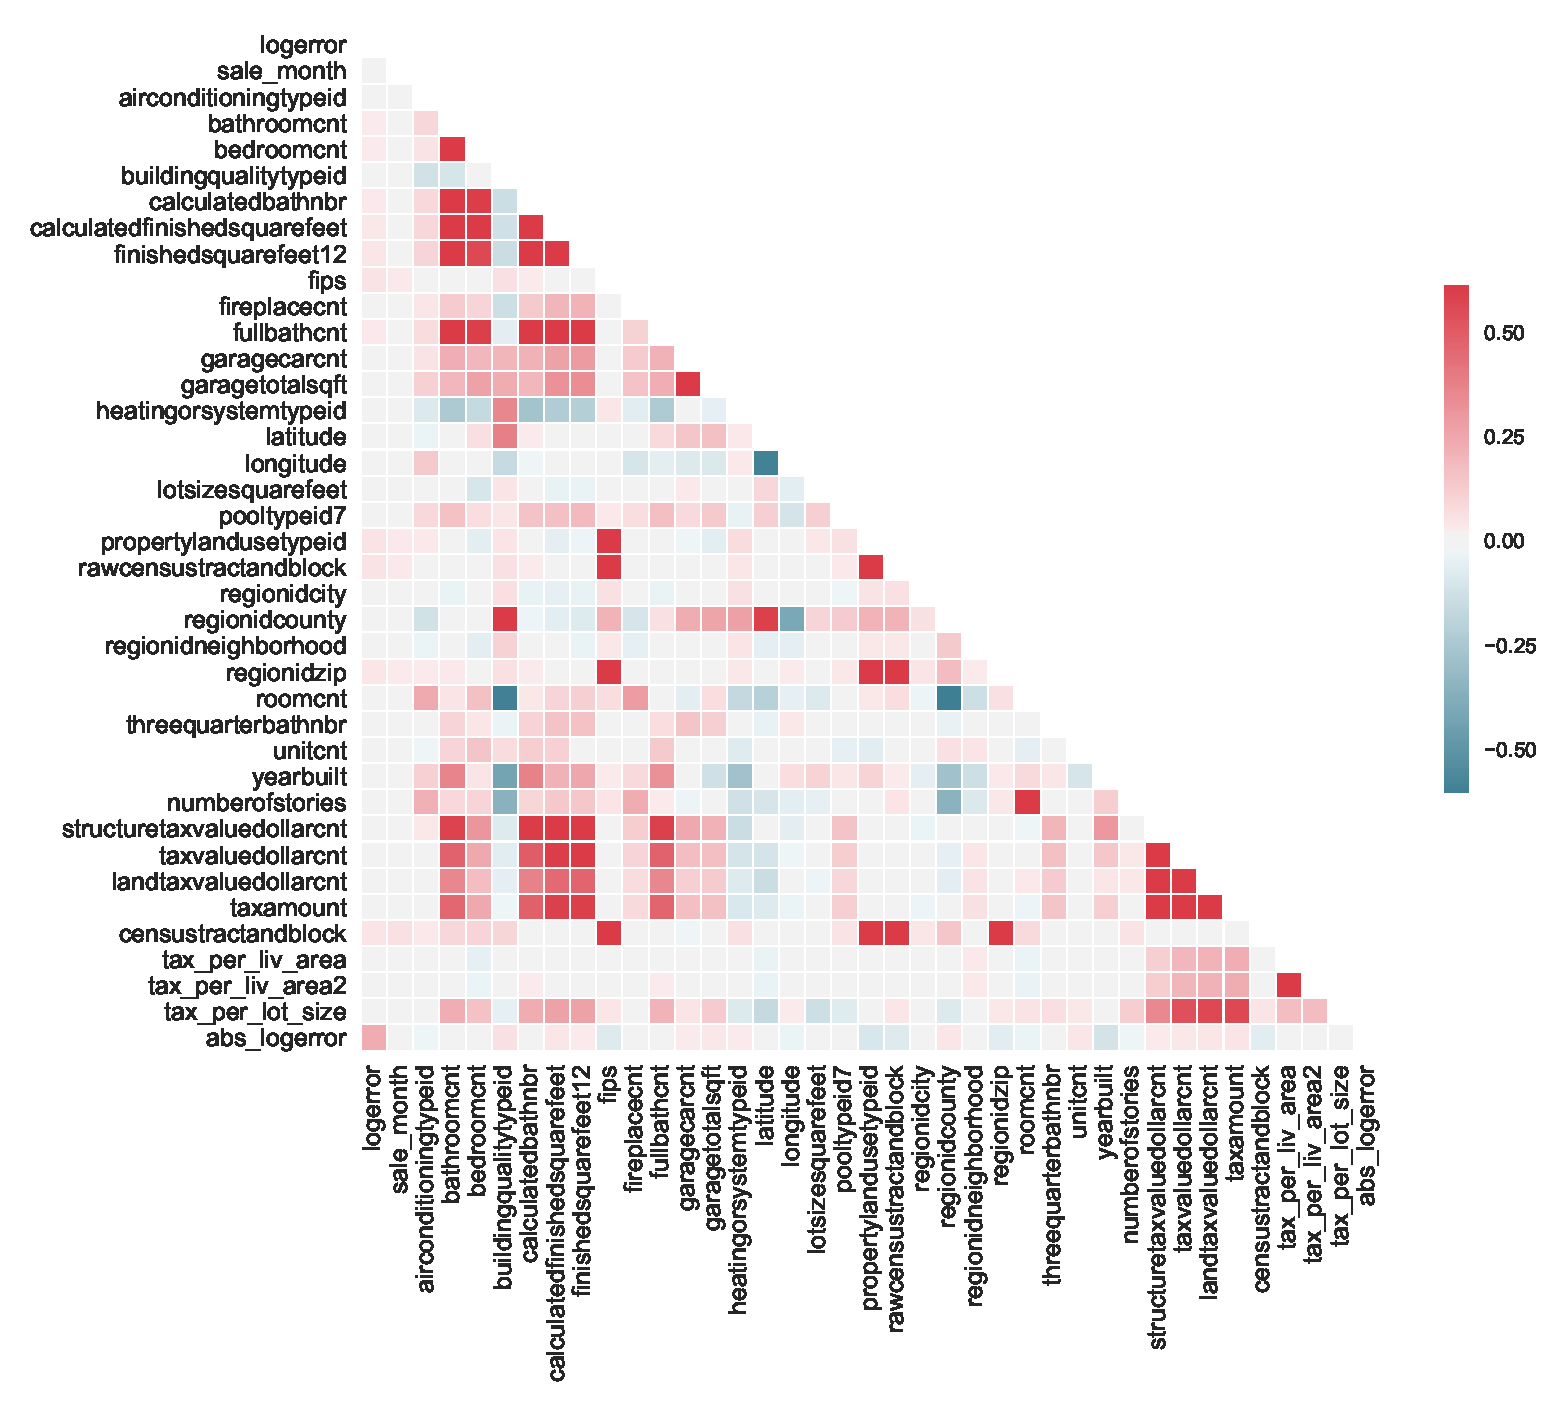
\includegraphics[width=1\linewidth]{pic/corr-train-data}
	\caption{The heatmap of the correlation coefficients among different features in the preprocessed dataset.}
	\label{fig:corr-train-data}
\end{figure}

\begin{figure}[!ht]
	\centering
	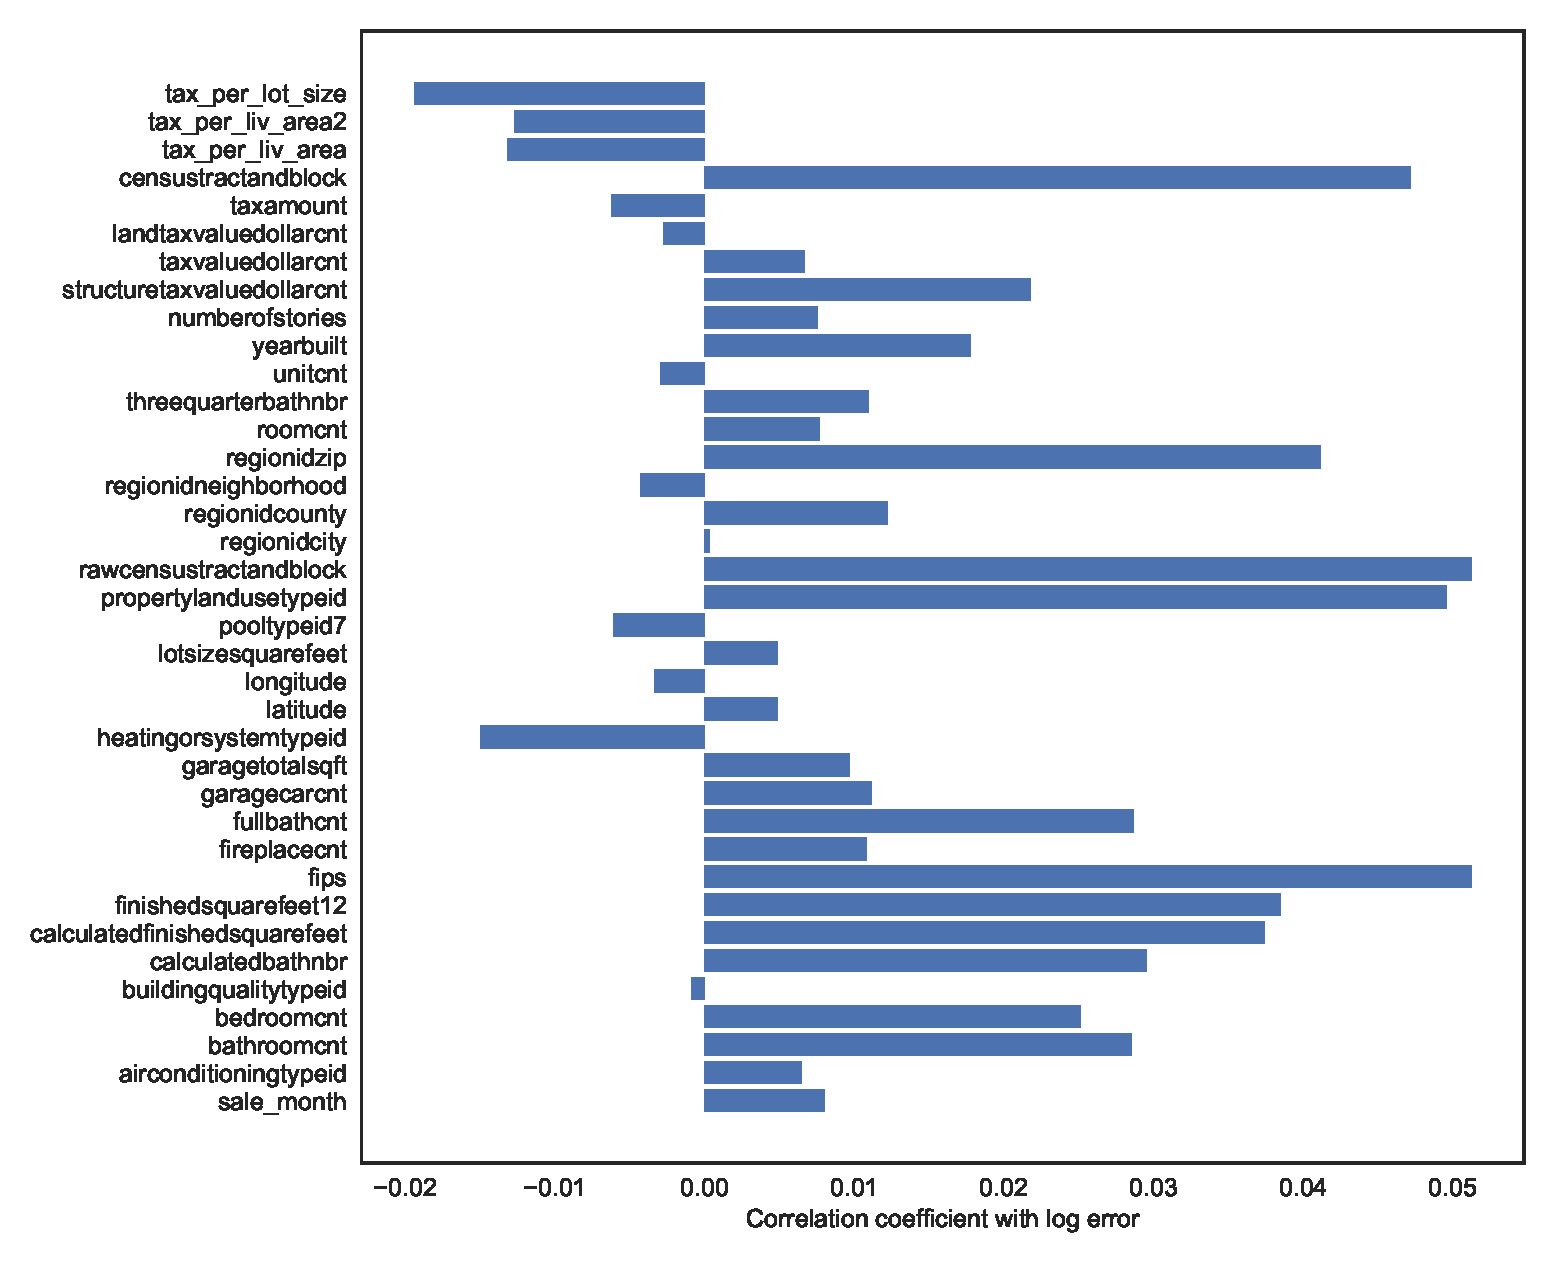
\includegraphics[width=1\linewidth]{pic/corr-features-vs-error}
	\caption{The correlation coefficients between $\xi_{\log}$ and other features.}
	\label{fig:corr-features-vs-error}
\end{figure}

\section{Methodology}\label{sec:methodology}
\subsection{Data preprocessing}
The workflow of data preprocessing can be divided into the following steps, which are given by 

For transaction dataset:
\begin{itemize}
	\item In the transaction dataset, create a feature named $sale\_month$ to store the month in which houses are sold. The value ranges from 1 to 12 to represent January to December. And drop the column named 'transcationdate'. 
\end{itemize}

For the properties dataset:

\begin{itemize}
	\item Remove the string features named 'propertycountylandusecode' and 'propertyzoningdesc' due to its high missing rate ($>90\%$) and difficulty to represent in regression model.
\end{itemize}

\begin{itemize}
	\item Handle missing values: Remove features with high percentage ($>90\%$) of missing values. Fill the missing values for features with relative low percentage ($\leq90\%$) of missing values. For categorical features, the most frequent value is filled, while the mean value is filled for continuously numerical feature. For features that are not continuously numerical like the count of bathrooms and bedrooms, the median values are filled.
\end{itemize}

\begin{itemize}
	\item Drop features with constant values.
\end{itemize}

%\begin{itemize}
%	\item Generate dummy vectors for categorical features as the additional features.
%\end{itemize}

\begin{itemize}
	\item Define three new features to consider the tax values per unit area of each house. The three features are defined by 
	\begin{equation}
		tax\_per\_liv\_area=taxamount/calculatedfinishedsquarefeet~\text{,}
	\end{equation}
	\begin{equation}
	tax\_per\_liv\_area2=taxamount/finishedsquarefeet12~\text{,}
	\end{equation}	
	\begin{equation}
	tax\_per\_lot\_size=taxamount/lotsizesquarefeet~\text{.}
	\end{equation}	
    where $taxamount$ is the total property tax assessed for that assessment year, $calculatedfinishedsquarefeet$ is calculated total finished living area of the home, $finishedsquarefeet12$ is finished living area, $lotsizesquarefeet$ is area of the lot in square feet.
\end{itemize}

\begin{itemize}
	\item Normalize all features to the scale from 0 to 1.
\end{itemize}

For the generation of the training and test dataset:
\begin{itemize}
	\item Merge the transaction and properties datasets according to the house ID (feature named $parcelid$) to generate the complete training dataset. The $parcelid$ is treated as row index not input feature.
\end{itemize}

\begin{itemize}
	\item The test dataset is the whole propties dataset as the input for the regression model. The $parcelid$ is treated as row index not input feature.
\end{itemize}

The heatmap of the correlation coefficients among different features in the preprocessed dataset is shown by Figure \ref{fig:corr-train-data}. As shown by Figure \ref{fig:corr-features-vs-error}, the correlation between $\xi_{\log}$ and other features demonstrates the possible important features to predict $\xi_{\log}$. More details will be discussed in Section \ref{sec:results}.

\subsection{Model implementation and refinement}
The linear regression, $k$-nearest neighbor, decision tree and random forest are implemented by the scikit learn packages. LightGBM are implemented by the packages provided on the related github pages (https://github.com/Microsoft/LightGBM). The GridSearchCV package from scikit learn is applied to optimize all five regression models. For the optimization of all regression models, the total training dataset is randomly separated into several groups of the training set and cross validation set. The score function is set as negative MAE.

The implementation (coding process) for each regression model can be summarized by the following several steps:

\begin{itemize}
	\item Implement data cleaning and generate the complete training dataset.
\end{itemize}

\begin{itemize}
	\item Apply the sciki-learn GridSearch package to optimize the chosen parameters for the best performance. During the optimization, the complete training dataset is randomly separated into training and cross validation datasets by the GridSearch package.
\end{itemize}

\begin{itemize}
	\item Train the regression model with the best parameters and the complete training set.
\end{itemize}

\begin{itemize}
	\item Predict $\xi_{\log}$ and output the final prediction.
\end{itemize}
The attached file Lightgbm.py is an example that shows the complete process which following the proposed steps to implement the LightGBM model.

Figure \ref{fig:linear_regression_opt}-\ref{fig:random_forest_opt} show the optimization results of different regression models including linear regression, $k$-nearest neighbors regression, decision tree regression and random forest regression. For linear regression, the ridge regression is applied and the best alpha for regularization strength is chosen as 0.02 for the best validation score. Similarly, for $k$-nearest neighbor regression, the best number of neighbors for averaging is chosen as 5. And the best maximum tree depth is chosen as 1 and 5 for decision tree and random forest regression, respectively. Applying the regular cross validation process by GridSearchCV packge, the LightGBM model is optimized by choosing the best learning rate (0.012).

\begin{figure}[!ht]
	\centering
	\includegraphics[width=0.9\linewidth]{pic/linear_regression_opt}
	\caption{The optimization curve (left) and training time (right) for linear regression model. For left panel, the black and red lines represent the training and validation curves, respectively. For right panel, the black and red lines represent the training and prediction time, respectively.}
	\label{fig:linear_regression_opt}
\end{figure}

\begin{figure}[!ht]
	\centering
	\includegraphics[width=0.9\linewidth]{pic/knn_opt}
	\caption{The optimization curve (left) and training time (right) for $k$-nearest neighbors regression model. For left panel, the black and red lines represent the training and validation curves, respectively. For right panel, the black and red lines represent the training and prediction time, respectively.}
	\label{fig:knn_opt}
\end{figure}

\begin{figure}[!ht]
	\centering
	\includegraphics[width=0.9\linewidth]{pic/decision_tree_opt}
	\caption{The optimization curve (left) and training time (right) for decision tree regression model. For left panel, the black and red lines represent the training and validation curves, respectively. For right panel, the black and red lines represent the training and prediction time, respectively.}
	\label{fig:decision_tree_opt}
\end{figure}

\begin{figure}[!ht]
	\centering
	\includegraphics[width=0.9\linewidth]{pic/random_forest_opt}
	\caption{The optimization curve (left) and training time (right) for random forest regression model. For left panel, the black and red lines represent the training and validation curves, respectively. For right panel, the black and red lines represent the training and prediction time, respectively.}
	\label{fig:random_forest_opt}
\end{figure}

\begin{figure}[!ht]
	\centering
	\includegraphics[width=0.9\linewidth]{pic/lightgbm_lr_opt}
	\caption{The optimization curve (left) for learning rate and training time (right) for LightGBM model. For left panel, the black and red lines represent the training and validation curves, respectively. For right panel, the black and red lines represent the training and prediction time, respectively.}
	\label{fig:lightgbm_lr_opt}
\end{figure}

\begin{table*}[!ht]
	\centering
	\footnotesize
	\caption{Scores for model evaluation}
	\label{tab:score-model-evaluation}
	\begin{tabular}{|c|c|c|}
		\hline model & training score  & test score\\  
		\hline  linear regression & -0.0693 & -0.0655\\
		\hline  $k$-nearest neighbor & -0.0720 & -0.0899\\
		\hline  decision tree & -0.0693 & -0.0654\\
		\hline  random forest & -0.0688  & -0.0653\\
		\hline  LightGBM & -0.0686  & -0.0650\\
		\hline  Median & -0.0690 & -0.0656\\
		\hline
	\end{tabular} 
\end{table*}

\section{Results}\label{sec:results}
\subsection{Model Evaluation}
The training and test scores (negative MAE) for the benchmark model and all different regression models are shown in Table \ref{tab:score-model-evaluation}. According to these scores, LightGBM has the best performance out of all different models. The performance of linear regression, decision tree and random forest are only slightly better than the benchmark model, while the $k$-nearest neighbor model performs has the worst performance. The reason may be that the size of the training dataset is not large enough to cover the complete range of then feature space. For outliers, the prediction by $k$-nearest neighbor model is not reliable. In general, the LightGBM model is chosen as the best model to predict $\xi_{\log}$ for this project.

\begin{figure}[!ht]
	\centering
	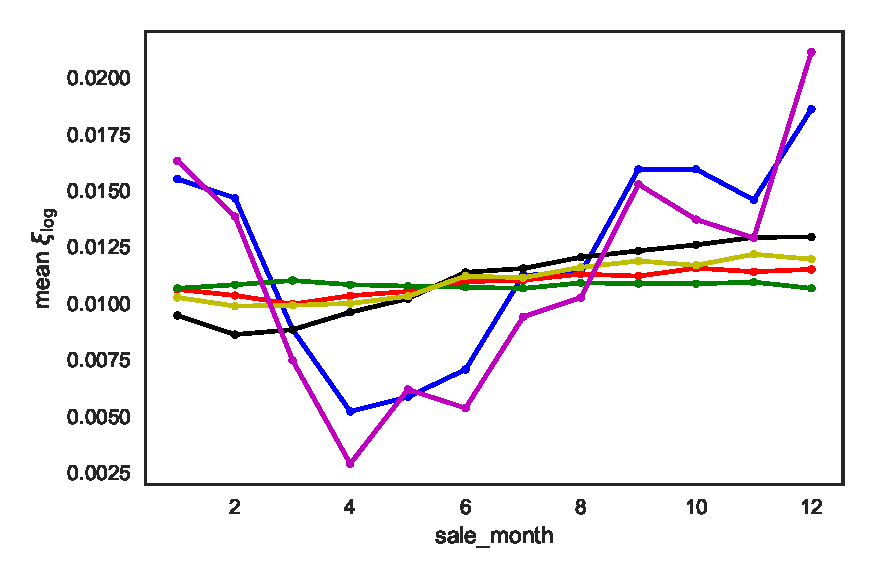
\includegraphics[width=0.9\linewidth]{pic/monthly-average-error-prediction}
	\caption{The comparison between real and predicted monthly average $\xi_{\log}$ of the training dataset. Legend: blue: exact $\xi_{\log}$, red: LightGBM, black: linear regression, green: decision tree, yellow: random forest, magenta: $k$-nearest neighbor }
	\label{fig:monthly-average-error-prediction}
\end{figure}


\begin{figure}[!ht]
	\centering
	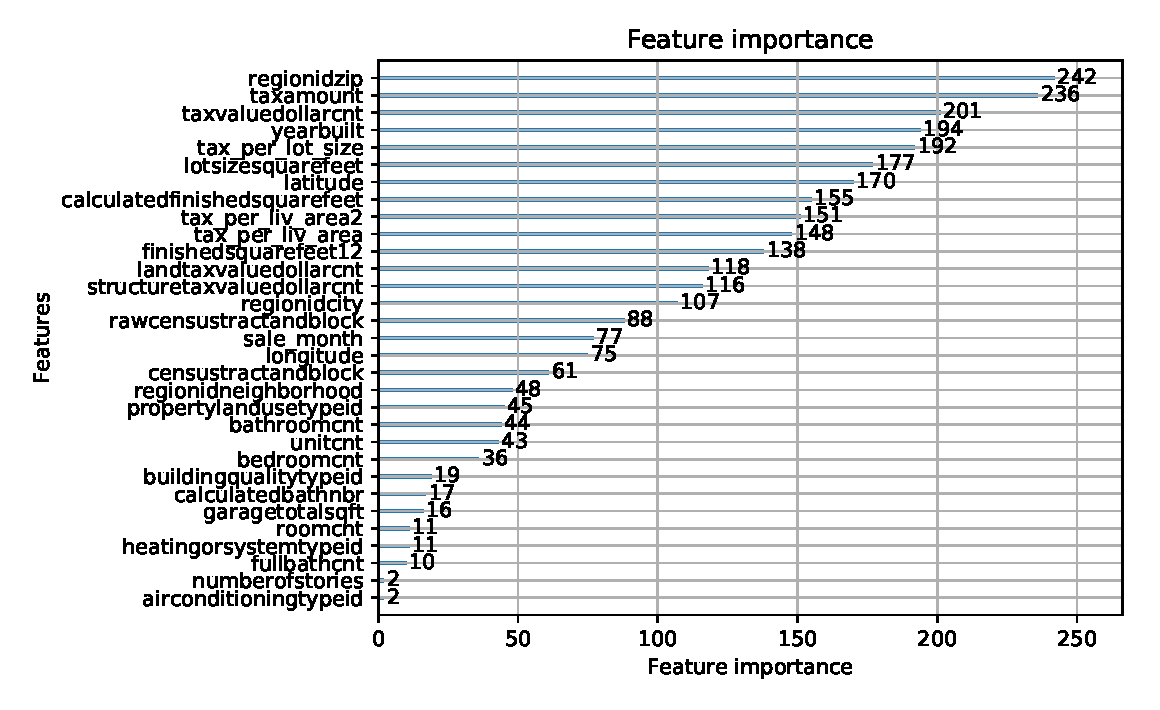
\includegraphics[width=0.9\linewidth]{pic/feature_importance}
	\caption{The importance of different features to predict log error based on the LightGBM model.}
	\label{fig:feature_importance}
\end{figure}

\begin{figure}[!ht]
	\centering
	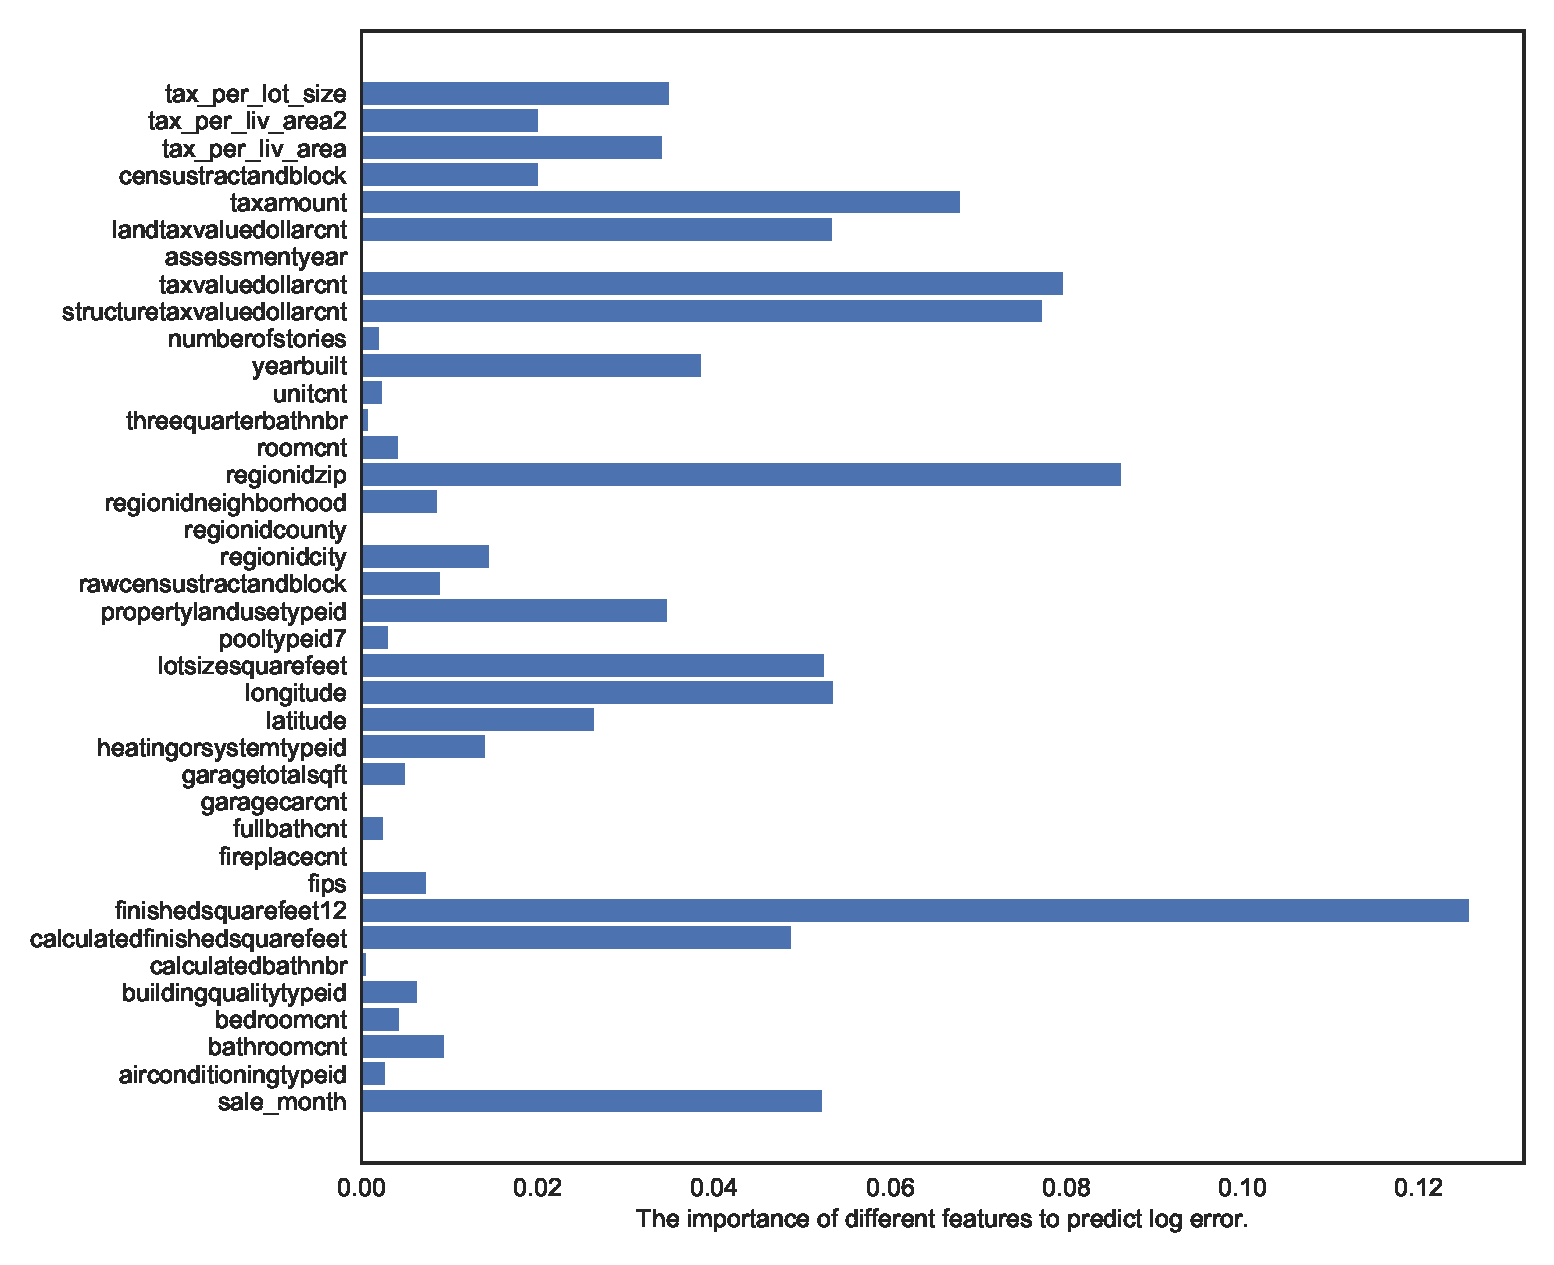
\includegraphics[width=0.9\linewidth]{pic/feature_importance_random_forest}
	\caption{The importance of different features to predict log error based on random forest regression model.}
	\label{fig:feature_importance_random_forest}
\end{figure}


\subsection{Validation and justification}
As shown by Figure {fig:monthly-average-error-prediction}, the monthly averaged $\xi_{\log}$ predicted by different regression models is compared to the training data. The prediction from linear regression, decision tree, random forest and LightGBM are similar. The LightGBM model tends to predict the median value of $\xi_{\log}$ from the training data to achieve less MAE. Compared to the benchmark model which applies the median value of $\xi_{\log}$ of the training dataset as the final prediction, the LightGBM model improves the prediction by decreasing 0.0006 MAE. This is a great improvement if considering the best score in the leaderboard of this Zillow competition on Kaggle platform is 0.0644, only 0.006 smaller than the score achieved by the proposed LightGBM model. In order to further validate the LightGBM model, a sensitivity test is conducted to test how predictions vary under the following methods to handle the missing values. The methods are given by

\begin{itemize}
	\item Method 1: fill all missing value as 0.
\end{itemize}

\begin{itemize}
	\item Method 2: fill all continuously numerical features as the mean values.
\end{itemize}

\begin{itemize}
	\item Method 3: fill all missing values as discussed in Section \ref{sec:methodology}.
\end{itemize}

The scores for the sensitivity test is shown by Table \ref{tab:score-sensitivity-test}. The variation in the performance of the LightGBM model is not obvious under different methods to handle missing values. This further validates that the prediction of the LightGBM model is reliable and stable. Furthermore, compared to the proposed data preprocessing, the LightGBM model has the same test score if Method 1 is applied (fill the missing values as 0). This indicates that the proposed data preprocessing by filling missing values with the mean, median and most frequent values of each feature may introduce noise and errors into the clean data and may not effectively improve model performance. 

\begin{table*}[!ht]
	\centering
	\footnotesize
	\caption{Scores for the sensitivity tests of the LightGBM model}
	\label{tab:score-sensitivity-test}
	\begin{tabular}{|c|c|c|}
		\hline method & training score & test score\\  
		\hline  1 & -0.0685 & -0.0650\\
		\hline  2 & -0.0685 & -0.0651\\
		\hline  2 & -0.0686 & -0.0650\\
		\hline
	\end{tabular} 
\end{table*}

\section{Conclusion}\label{sec:conclusion}
\subsection{Project summary}
In this project, the Zillow dataset for the Kaggle competition is visualized, analyzed and applied to predict $\xi_{\log}$ between the real sale price and the Zillow 'Zestimate'. A complete exploratory analysis on both the transaction and properties datasets has been conducted to indicate the possible relationship between $\xi_{\log}$ and different features. Meanwhile, a reasonable data preprocessing has been conducted to clean the dataset, while different regression models have been optimized to accurately predict $\xi_{\log}$. Compared to other regression models, since the LightGBM performs best without any compromise in both accuracy and efficiency, it is chosen as the best model to predict $\xi_{\log}$ in this project.

\subsection{Feature importance}
In order to demonstrate the key factors in predicting $\xi_{\log}$, the importance of different features based on the LightGBM model is shown by Figure \ref{fig:feature_importance}. According to this Figure, the zip code, property tax, house lot size and yearbuilt are the most important features. This is further validated by the random forest model that has the similar pattern of the distribution of feature importance (Figure \ref{fig:feature_importance_random_forest}). This indicates that the original algorithm of 'Zestimate' need to be improved on the representation of these features on predicting house sale price. Starting from this point, different sensitivity tests and parameter tuning can be conducted to increase the reliability of the 'Zestimate' model when the original algorithm of 'Zestimate' is accessible.

\subsection{Improvement}
Compared to the best score (lowest MAE) 0.0644 on the leaderboard of this competition, the performance of the LightGBM model can still be improved from many aspects. Here are some possible ways:

\begin{itemize}
	\item Involve more features: Due to the high missing rate, more than 40\% features is removed although the cutoff percentage is set as high as 90\%. If the information from removed features can be still used, it may improve the performance of the LightGBM model.  
\end{itemize}

\begin{itemize}
	\item Better missing values: Currently, the missing values are filled with the mean, median and most frequent values for different features. This may be not reasonable since some known features may relate to the feature with missing values. A better missing values should be predicted by the know information from each house. For example, if latitude and longitude are known, and the zip code is not known, the missing zip code should be filled with the exact value based on the geographical information, not the most frequent zip code.
\end{itemize}

\begin{itemize}
	\item Create more features: In this project, three new features are created to improve regression models. According to the feature importance (Figure \ref{fig:feature_importance} and \ref{fig:feature_importance_random_forest}), they are all important to predict $\xi_{\log}$. More reasonable new features can be created to improve model performance. 
\end{itemize}

\begin{itemize}
	\item Parameter tuning: The LightGBM model has many parameter to choose for best performance. In this project, only the optimization of learning rate is conducted. More cross validation process is required to achieve better parameters from the model.
\end{itemize}

\begin{itemize}
	\item Boosting with other models: The LightGBM model is a gradient boosting framework using tree based learning algorithm. In order to achieve better performance, the same boosting technique can be applied to combine the results from different regression models.
\end{itemize}

\end{document}